%%
%% Author: papian
%% 26/05/18
%%



\documentclass{bredelebeamer}




%%%%%%%%%%%%%%%%%%%%%%%%%%%%%%%%%%%%%%%%%%%%%%%%



\title[OS Project]{Operating System Project}
% Titre du diaporama

\subtitle{An implementation of server-client database using non-blocking operations}
% Sous-titre optionnel

\author{Julmy, S., Papinutto, M. \& Veillard, S.}
% La commande \inst{...} Permet d'afficher l' affiliation de l'intervenant.
% Si il y a plusieurs intervenants: Marcel Dupont\inst{1}, Roger Durand\inst{2}
% Il suffit alors d'ajouter un autre institut sur le modèle ci-dessous.

\institute[UniFr]{}


\date{30 Septembre 2018}
% Optionnel. La date, généralement celle du jour de la conférence

\subject{Presentation projet OS Group 4 Sylvain Julmy, Michael Papinutto et Sami Veillard}
% C'est utilisé dans les métadonnes du PDF

\logo{
\includegraphics[scale=0.5]{../report/images/unifrlogo.jpg}}

%%%%%%%%%%%%%%%%%%%%%%%%%%%%%%%%%%%%%%%%%%%%%%%%%%%%%%%%%%%%%%%%%%%%%
\begin{document}

    \begin{frame}
        \titlepage
    \end{frame}

    \begin{frame}{Sommaire}
        \tableofcontents
        % possibilité d'ajouter l'option [pausesections]
    \end{frame}

    \section{Selected Approach}

    \begin{frame}{Multi-threaded Server}
        We selected a multi-threaded server as: \\
        \begin{itemize}
            \item Allows to access same data structure
            \item light weight as compared to multi-process server
            \item easier to implement
        \end{itemize}
    \end{frame}

     \begin{frame}{To use Mutex or not to use Mutex}

         Our lock-free implementation allowed us not to use Mutex \\

        \begin{itemize}
            \item No need to prioritize read or write operations
            \item No deadlock problems
            \item All clients have the same right to access the data structure at any time
        \end{itemize}
    \end{frame}

     \begin{frame}{non-blocking operations}

        Non-blocking operations use atomic operations allowing to perform several action at each clock cycle\\
        As the actions are perform in a single cycle it is not crucial to wait for the operation to be completed \\
        In C, atomic operations functionality such as CompareAndSet can be done by "stealing" a bit from a pointer
        using bit-wise operators to extract the pointer and the mark from a single word \\

        \begin{itemize}
            \item Swap values example
        \end{itemize}
    \end{frame}

     \begin{frame}{Reversed Split-Ordered Hash-Set}
        This implementation offers a rapid access to the data but might require slightly more memory that other data-structure
        \begin{itemize}
            \item Buckets are linked to a stack as the list grows supplemental buckets references are added so that buckets is keep small
            \item Require to set up sentinel bucket in order to avoid "corner case" that occurs when deleting a reference by a bucket reference
            \item The sentinel bucket is never deleted
        \end{itemize}
         \begin{figure}
             \centering
             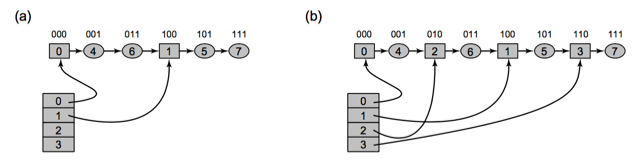
\includegraphics{../report/images/hashsetFig1.png}
         \end{figure}
    \end{frame}

     \begin{frame}{Operation add in this Hash-Set}
         Scheme of the procedure that add the key 10 to the lock-free hash-set
         \begin{figure}
             \centering
             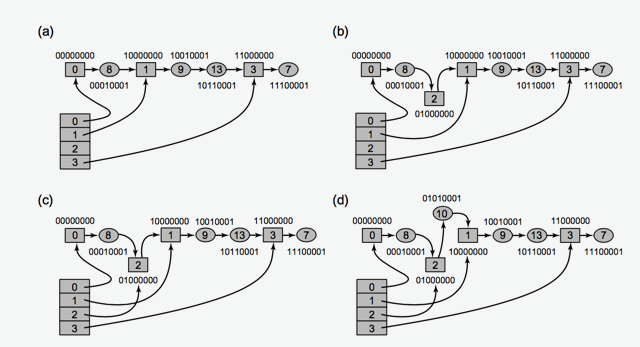
\includegraphics{../report/images/hashsetFig2.png}
         \end{figure}
    \end{frame}

    \section{Usage and Graphical User Interface}

     \begin{frame}{Program Basic Usage}
         \begin{tcolorbox}[taborange,tabularx={X|Y}, boxrule=3pt, title=Server usage]
            TCP Port & 5000 (can be changed in file) \\\hline
            .\textbackslash server & server start
         \end{tcolorbox}
         \begin{tcolorbox}[tabvert,tabularx={X|Y}, boxrule=3pt, title=Client Start]
            .\textbackslash client <server ip address> & client start \\\hline
            .\textbackslash client -option <server ip address> & client start with options
         \end{tcolorbox}
    \end{frame}
    \begin{frame}{Client Usage and Commands}
          \begin{tcolorbox}[tabbleu,tabularx={X|Y}, boxrule=3pt, title=Client Special Starts]
              {-? \\ -h \\ -{}-help} & client command help \\\hline
            {-f <file> \\ -{}-file <file>} & client start and execute commands in the file \\\hline
            {-F <file1> \ldots <fileN> \\ -{}-files <file1> \ldots <fileN>} & client start and execute commands in the files \\
         \end{tcolorbox}
         \begin{tcolorbox}[tabvert,tabularx={X|Y}, boxrule=3pt, title=Commands in interactive GUI]
             add <value> or add <key> <value> & add a value to the database  \\\hline
            ls & list content (unordered) \\\hline
            read\_v <key> & read value from  key \\\hline
            read\_k <value> & read key from value \\\hline
            rm\_v <key> & delete value from key \\\hline
            rm\_k <value> & delete value from key \\\hline
            update\_kv <value> <newvalue> & update an entry
         \end{tcolorbox}
    \end{frame}

    \begin{frame}{Demo}
        \boitebleue{\begin{center}
                     DEMO
        \end{center}}
    \end{frame}


    \section{Tests}
    \begin{frame}{Tests scenarios}
        We tested the following scenarios:
        \begin{itemize}
            \item Collisions scenario : Operations that can collide (a client delete a value before another access it)
            \item No-Collisions scenario : Operations that are order so that no collision can occurs
            \item Many client: several client with similar scenario as no-collisions
        \end{itemize}
    \end{frame}

     \begin{frame}{Collision scenario}
         We tested 11 clients and 28 commands (308 operations in total)
         \begin{tcolorbox}[tabrouge,tabularx={X|Y|Y|Y}, boxrule=3pt]
               & Add & Read & Delete\\\hline
               Number of errors & 0 & 22 & 0 \\\hline
               Percentage of errors & 0\% & 7.14\% & 0\%
         \end{tcolorbox}
    \end{frame}
     \begin{frame}{No-collision scenario}
         We tested 8 clients and 2700 commands (21600 operations in total)
         \begin{tcolorbox}[taborange,tabularx={X|Y|Y|Y}, boxrule=3pt]
               & Add & Read & Delete\\\hline
               Number of errors & 0 & 0 & 0 \\\hline
               Percentage of errors & 0\% & 0\% & 0\%
         \end{tcolorbox}
    \end{frame}
         \begin{frame}{Many clients scenario}
         We tested 32 clients and 300 commands (9600 operations in total)
         \begin{tcolorbox}[taborange,tabularx={X|Y|Y|Y}, boxrule=3pt]
               & Add & Read & Delete\\\hline
               Number of errors & 0 & 0 & 0 \\\hline
               Percentage of errors & 0\% & 0\% & 0\%
         \end{tcolorbox}
         This last test required more time than the previous one despite it has half less operations
    \end{frame}

    \section{Final}
    \begin{frame}
        \centering
        \textcolor{MidnightBlue}{\Huge Thank you for your attention !}

    \end{frame}
\end{document}
